\section{Menghavan 12: Inchor\'{a}n\'{e} Rh\'{e}iach \textendash\ Inchor\'{a}n\'{e} hAnr\'{e}iach}
(\textit{Lesson 12: Direct Clauses \textendash\ Indirect Clauses})\\

In the twelfth lesson you will learn what direct and indirect clauses are, and how they are constructed in Gal\'{a}thach.

\subsection{Gwepchoprith: Conversation}

\subsubsection{Conversation}

Below are two conversations between three people. Tarchonwoth is a man, Tuthch\'{a}na and Cunv\'{a}ra are women. All three are attested Gaulish names. These conversations show you how direct clauses and indirect clauses are constructed.

%\tcbox[colback=red!10!green!10, colframe=green!20!black!80]
\begin{table}[H]
\centering
    \begin{tabular}{cM{10.0cm}c}
    \cellcolor{lightgreen} & \cellcolor{lightgreen} & \cellcolor{lightgreen}\\
    \cellcolor{lightgreen}\textcolor{darkgreen}{\textbf{Tarchonwoth}} & \cellcolor{lightgreen} & \cellcolor{lightgreen}\textcolor{darkgreen}{\textbf{Tuthch\'{a}na}}\\
    \cellcolor{lightgreen} & \cellcolor{lightgreen} & \cellcolor{lightgreen}\\
    \cellcolor{lightgreen} & \cellcolor{lightgreen} & \cellcolor{lightgreen}\\
    \cellcolor{lightgreen} & \cellcolor{lightgreen} & \cellcolor{lightgreen}\\
    \cellcolor{lightgreen} & \cellcolor{lightgreen} & \cellcolor{lightgreen}\\
    \cellcolor{lightgreen} & \cellcolor{lightgreen} & \cellcolor{lightgreen}\\
    \cellcolor{lightgreen} & \cellcolor{lightgreen} & \cellcolor{lightgreen}\\
    \cellcolor{lightgreen}\multirow{-7}{*}{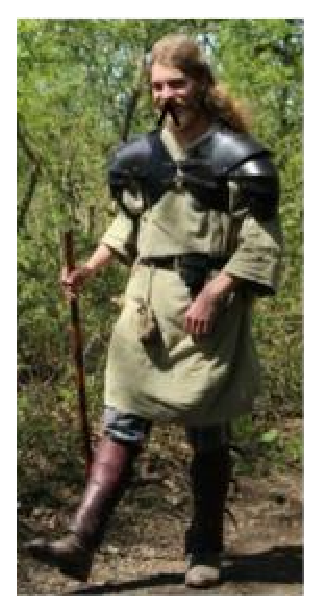
\includegraphics[height=4.0cm]{img/menghavan12_1}} & \cellcolor{lightgreen} & \cellcolor{lightgreen}\multirow{-7}{*}{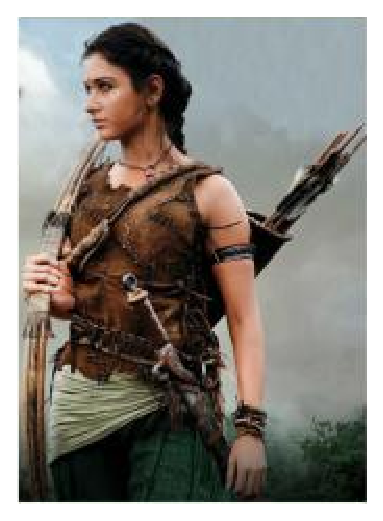
\includegraphics[height=4.0cm]{img/menghavan12_2}}\\
    \cellcolor{lightgreen} & \cellcolor{lightgreen} & \cellcolor{lightgreen}
    \end{tabular}
\end{table}

\begingroup
\fontsize{10pt}{12pt}\selectfont
\begin{leftbubbles}D\'{\i} wath, p\'{e} gaman a hesi ti?\end{leftbubbles}
\begin{rightbubbles}
D\'{\i} wath adhith c\'{o}\'{e}th.

Esi mi in dh\'{a}i, br\'{a}thu.

Ach ti-s\'{u}\'{e}?
\end{rightbubbles}
\begin{leftbubbles}Esi mi in dh\'{a}i c\'{o}\'{e}th.\end{leftbubbles}
\begin{rightbubbles}Gwerthamich.\end{rightbubbles}
\begin{leftbubbles}
Gw\'{e}la mi prin \'{e}p.

A ghn\'{\i}a ti don nep o g\'{a}la \'{e} rin\'{o}thi \'{e}p adhim?
\end{leftbubbles}
\begin{rightbubbles}
Gn\'{\i}a mi.

Gn\'{\i}a mi ben shen o g\'{a}la \'{o} d\'{u}ithir rin\'{o}thi \'{e}p adhith.

Esi \'{o} anu Cunv\'{a}ra.

\'{A}i a gantha hal in bron ach p\'{e}tha adh\'{\i} ins\'{e}.
\end{rightbubbles}
\begin{leftbubbles}Br\'{a}thu r\'{e} h\'{e}lu, esi ti r\'{e} chw\'{o}rethw\'{a}r.\end{leftbubbles}
\begin{rightbubbles}Esi \'{\i} m\'{o} har\'{u}er im\'{\i}. Esi \'{\i} neveth.\end{rightbubbles}
\endgroup

\begin{center}\textcolor{darkgray}{\textit{\'{A}ia Tarchonwoth a h\'{a}pis in ven shen a gantha hal in bron.}}\end{center}

\begin{table}[H]
\centering
    \begin{tabular}{cM{10.0cm}c}
    \cellcolor{lightgreen} & \cellcolor{lightgreen} & \cellcolor{lightgreen}\\
    \cellcolor{lightgreen}\textcolor{darkgreen}{\textbf{Tarchonwoth}} & \cellcolor{lightgreen} & \cellcolor{lightgreen}\textcolor{darkgreen}{\textbf{Cunv\'{a}ra}}\\
    \cellcolor{lightgreen} & \cellcolor{lightgreen} & \cellcolor{lightgreen}\\
    \cellcolor{lightgreen} & \cellcolor{lightgreen} & \cellcolor{lightgreen}\\
    \cellcolor{lightgreen}\multirow{-3}{*}{
\includegraphics[height=2.0cm]{img/menghavan12_3}} & \cellcolor{lightgreen} & \cellcolor{lightgreen}\multirow{-3}{*}{
\includegraphics[height=2.0cm]{img/menghavan12_4}}\\
    \cellcolor{lightgreen} & \cellcolor{lightgreen} & \cellcolor{lightgreen}
    \end{tabular}
\end{table}

\begin{leftbubbles}D\'{\i} wath. A hesi \'{\i} ti-s\'{u}\'{e} o t\'{o} dh\'{u}ithir \'{\i}-esi \'{e}p a brin?\end{leftbubbles}
\begin{rightbubbles}
Esi \'{\i} mi-s\'{u}\'{e}.

A chw\'{e}la ti \'{a}pis in \'{e}p o g\'{a}la m\'{o} dh\'{u}ithir rin\'{o}thi ich\'{\i}?
\end{rightbubbles}
\begin{leftbubbles}In chw\'{\i}r, gw\'{e}la mi.\end{leftbubbles}
\begin{rightbubbles}Esi \'{e} ins\'{e}, derchi. A harw\'{e}ra \'{e} adhith?\end{rightbubbles}
\begin{center}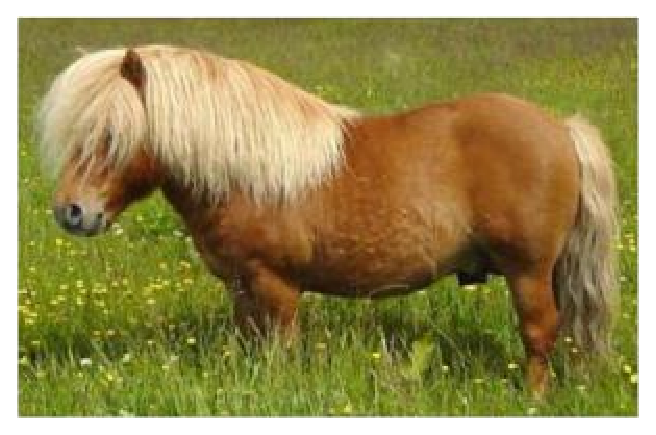
\includegraphics[height=4.0cm]{img/menghavan12_5}\end{center}

\newpage
\subsubsection{Colav\'{a}ru \textendash\ Tr\'{e}lav\'{a}ru}
(Conversation \textendash\ Translation)

Tarchonwoth: D\'{\i} wath, p\'{e} gaman a hesi ti?\\
(Tarchonwoth: Good day, how are you?)\\

Tuthch\'{a}na: D\'{\i} wath adhith c\'{o}\'{e}th. Esi mi in dh\'{a}i, br\'{a}thu. Ach ti-s\'{u}\'{e}?\\
(Tuthch\'{a}na: Good day to you too. I am well, thank you. And yourself?)\\

Tarchonwoth: Esi mi in dh\'{a}i c\'{o}\'{e}th.\\
(Tarchonwoth: I am well too.)\\

Tuthch\'{a}na: Gwerthamich.\\
(Tuthchana: Excellent.)\\

Tarchonwoth: Gw\'{e}la mi prin \'{e}p. A ghn\'{\i}a ti don nep o g\'{a}la \'{e} rin\'{o}thi \'{e}p adhim?\\
(Tarchonwoth: I want to buy a horse. Do you know any person who can sell a horse to me?)\\

Tuthch\'{a}na: Gn\'{\i}a mi. Gn\'{\i}a mi ben shen o g\'{a}la \'{o} d\'{u}ithir rin\'{o}thi \'{e}p adhith. Esi \'{o} anu Cunv\'{a}ra. \'{a}i a gantha hal in bron ach p\'{e}tha adh\'{\i} ins\'{e}.\\
(Tuthch\'{a}na: I do. I know an old woman whose daughter can sell a horse to you. Her name is Cunvara. Go to the other side of the hill and ask her there.)\\

Tarchonwoth: Br\'{a}thu r\'{e} h\'{e}lu, esi ti r\'{e} chw\'{o}rethw\'{a}r.\\
(Tarchonwoth: Thanks very much, you're very helpful.)\\

Tuthch\'{a}na: Esi \'{\i} m\'{o} har\'{u}er im\'{\i}. Esi \'{\i} neveth.\\
(Tuthch\'{a}na: It's my pleasure. It's nothing.)\\

$[$\'{A}ia Tarchonwoth a h\'{a}pis in ven shen a gantha hal in bron.$]$\\

Tarchonwoth: D\'{\i} wath. A hesi \'{\i} ti-s\'{u}\'{e} o t\'{o} dh\'{u}ithir \'{\i}-esi \'{e}p a brin?\\
(Tarchonwoth: Good day. Is it yourself whose daughter has a horse to buy?)\\

Cunv\'{a}ra: Esi \'{\i} mi-s\'{u}\'{e}. A chw\'{e}la ti \'{a}pis in \'{e}p o g\'{a}la m\'{o} dh\'{u}ithir rin\'{o}thi ich\'{\i}?\\
(Cunv\'{a}ra: It is myself. Do you want to see the horse that my daughter can sell?)\\

Tarchonwoth: In chw\'{\i}r, gw\'{e}la mi.\\
(Tarchonwoth: Yes, I do.)\\

Cunv\'{a}ra: Esi \'{e} ins\'{e}, derchi. A harw\'{e}ra \'{e} adhith?\\
(Cunv\'{a}ra: It is there, look. Does it please you?)\\

\subsubsection{Vocabulary}

\begin{table}[H]
\centering
\begin{tabular}{cc}
  \toprule
  \textbf{Gal\'{a}thach} & \textbf{English}\\
  \cmidrule(lr){1-1}\cmidrule(lr){2-2}
  gwerthamich & excellent\\
  prin & to buy\\
  don nep & any/some person\\
  rin\'{o}thi & to sell\\
  ben & woman\\
  sen & old\\
  d\'{u}ithir & daughter\\
  cantha & side\\
  al & other\\
  bron & hill\\
  derchi & to look\\
  \bottomrule
\end{tabular}
\label{vocab_conversation_lesson12}
\caption{Vocabulary conversation lesson 12}
\end{table}

\subsection{Gwepchoprith: Direct clauses}

\subsubsection{Direct clauses}
A direct clause is a part of a sentence that refers back to the subject of the previous part of the sentence.

\begin{quote}
  \textit{this is the man who wants to buy a horse}
\end{quote}

The direct clause is \textit{who wants to buy a horse}. The word \textit{who} refers to \textit{the man}, which was the subject of the previous part of the sentence \textit{this is the man}.

In Gal\'{a}thach there are four ways of constructing this sentence.

\subsubsection{Introducing the clause with the word \textit{o} and not restating the subject}

The word ``o'' means \textit{that} or \textit{which}. If it is followed by a word that starts with a vowel it becomes ``och''.

\begin{table}[H]
\centering
\begin{tabular}{cc}
  \toprule
  \textbf{Gal\'{a}thach} & \textbf{English}\\
  \cmidrule(lr){1-1}\cmidrule(lr){2-2}
  esi & is\\
  sin & this\\
  in gwir & the man\\
  o & that (which)\\
  gwel & to want\\
  prin & to buy\\
  in \'{e}p & the horse\\
  esi sin in gwir o gw\'{e}la prin in \'{e}p & this is the man who wants to buy the horse\\
  \bottomrule
\end{tabular}
\label{examples_way1}
\end{table}

The word \textit{o} connects the two phrases and refers to \textit{the man}. There is no confusion because there is no other word in the second phrase that can be interpreted as a subject:

\begin{quote}
gw\'{e}la prin in \'{e}p (want buying the horse)
\end{quote}

The word \textit{\'{e}p} can not be interpreted as a subject because it does not follow the verb immediately. In this case there is no need to restate the subject.

\subsubsection{Introducing the clause with the word \textit{o} and restating the subject}

This is necessary when there can be confusion about which is the subject of the second phrase.

\begin{quote}
esi sin in gwir o gw\'{e}la in \'{e}p
\end{quote}

This sentence can be interpreted in two ways:
\begin{itemize}
    \item this is the man who wants the horse
    \item this is the man who the horse wants
\end{itemize}

Because the words \textit{in \'{e}p}, \textit{the horse} follow directly after the verb, they can be interpreted as being the subject of the second verb \textit{gwel}, \textit{wanting}.

Therefore the subject needs to be restated with a pronoun that refers back to the subject of the first phrase. This is called using a resumptive pronoun.

\begin{quote}
esi sin in gwir o gw\'{e}la \'{e} in \'{e}p (this is the man who wants the horse)
\end{quote}

The literal translation of this sentence is \textit{this is the man that he wants the horse}.

In reality the direct clause becomes a subordinate clause linked to the main clause with the word \textit{o}.

\subsubsection{Linking the second clause to the first clause with the suffix \textit{-i\'{o}} which gets attached to the end of the verb of the second clause}

\begin{quote}
esi sin in gwir gweli\'{o} in \'{e}p (this is the man who wants the horse)
\end{quote}

The suffix \textit{-i\'{o}} always refers back to the subject immediately in front of it. The literal translation of this sentence is something like \textit{this is the man wanting the horse}.

\subsubsection{Linking the second clause to the first clause with the preposition \textit{en} in front of the verb}

This causes initial consonant mutation on the verb. The verb is in the root or infinitive form.


\begin{quote}
esi sin in gwir en chwel in \'{e}p
\end{quote}

The literal translation of this sentence is \textit{this is the man wanting the horse}. It is the same as using the suffix \textit{-i\'{o}}.

Because the verb is in the root or infinitive form there can be no confusion about what is the subject of the second clause, because a subject can never follow a verb in the root or infinitive form.

Using the preposition \textit{en} to link a second clause to a main clause can only be done in the present tense.\\
People choose freely from these four ways of constructing direct clauses. However, the second one (b) is the easiest one.

\subsection{Gwepchoprith: Indirect clauses}
\subsubsection{Indirect clauses}

A direct clause is a part of a sentence that refers back to the subject of the previous part of the sentence, but in an indirect way.

\begin{quote}
  \textit{this is the man whose daughter wants to buy the horse}
\end{quote}

The second clause starts with ``whose daughter''. The words ``whose daughter'' refer back to the subject of the previous clause, but the actual subject of the second clause is the daughter, not the man himself.

In Gal\'{a}thach there is only one way to construct this sentence. The clause is introduced with the word \textit{o} and the subject is stated independently. The subject becomes \textit{his daughter}.

esi sin in gwir o gw\'{e}la \'{o} dh\'{u}ithir prin in \'{e}p

The literal translation of this sentence is \textit{this is the man that his daughter wants to buy the horse}. As above in Direct Clauses (b) the clause becomes a subordinate clause with its own independent subject, linked to the first clause with the word \'{o}.

\newpage
\subsection{Exercises}

\subsubsection{Vocabulary}

\begin{table}[H]
\centering
\begin{tabular}{cc}
  \toprule
  \textbf{Gal\'{a}thach} & \textbf{English}\\
  \cmidrule(lr){1-1}\cmidrule(lr){2-2}
  cath & cat\\
  can\'{\i}ath & singer\\
  druch & bad\\
  mapath & child\\
  depri & to eat\\
  grau & sand\\
  lavar & to talk\\
  i\'{o}inch & young\\
  derchi & to look (at)\\
  r\'{e}dhi & to ride\\
  m\'{e}i & little\\
  geneth & girl\\
  d\'{a}thr\'{a}ieth & feet (one pair)\\
  calw\'{a}r & boot\\
  mer & crazy\\
  l\'{\i}auth & shape\\
  t\'{o}i & bow\\
  c\'{a}th\'{o}i & arrow\\
  d\'{o}s & arm\\
  s\'{\i}r & long\\
  nerthach & strong\\
  \bottomrule
\end{tabular}
\label{vocab_indirect_clauses}
\end{table}

\subsubsection{Translate}

Translate the following phrases:

\begin{table}[H]
\centering
\begin{tabular}{|c|M{5.0cm}|}
  \toprule
  \textbf{English} & \textbf{Gal\'{a}thach}\\
  \toprule
  That is the woman who talks to cats & \\
  \midrule
  Here is the man who is a bad singer & \\
  \midrule
  This the child that eats sand & \\
  \midrule
  Cunv\'{a}ra is the old woman who talks to Tarchonwoth & \\
  \midrule
  Tarchonwoth is the young man who looks at Tuthch\'{a}na & \\
  \midrule
  Tuthch\'{a}na is the girl whose sister rides little horses & \\
  \midrule
  Tarchonwoth is the man whose feet are in boots & \\
  \midrule
  Cunv\'{a}ra is the woman whose eyes are crazy & \\
  \midrule
  It is the horse whose legs are in excellent shape & \\
  \midrule
  There goes the woman with the bow and arrows whose arms are long and strong & \\
  \bottomrule
\end{tabular}
\label{exercise_indirect_clauses}
\caption{Exercise: indirect clauses}
\end{table}

\newpage
\subsubsection{Solution}
\begin{table}[H]
\centering
\rotatebox{180}{%
  \begin{tabular}{|c|>{\itshape}c|}
  \toprule
  \textbf{English} & \textbf{Gal\'{a}thach}\\
  \toprule
  That is the woman who talks to cats & Esi s\'{e} in ven o lav\'{a}ra can g\'{a}th\'{e}.\\
  \midrule
  Here is the man who is a bad singer & Insin esi in gwir och esi \'{e} can\'{\i}ath druch.\\
  \midrule
  This the child that eats sand & Esi sin in mapath o depra \'{e} grau.\\
  \midrule
  Cunv\'{a}ra is the old woman who talks to Tarchonwoth & Esi Cunv\'{a}ra in ven shen en lhavar can Tarchonwoth.\\
  \midrule
  Tarchonwoth is the young man who looks at Tuthch\'{a}na & Esi Tarchonwoth in gwir i\'{o}inch derchi\'{o} Tuthch\'{a}na.\\
  \midrule
  Tuthch\'{a}na is the girl whose sister rides little horses & Esi Tuthch\'{a}na in gheneth o r\'{e}dha \'{o} sw\'{\i}or \'{e}p\'{e} m\'{e}i.\\
  \midrule
  Tarchonwoth is the man whose feet are in boots & Esi Tarchonwoth in gwir och esi \'{o} dh\'{a}thr\'{a}ieth en galw\'{a}r\'{e}.\\
  \midrule
  Cunv\'{a}ra is the woman who has crazy eyes & Esi Cunv\'{a}ra in ven och \'{\i}-esi d\'{a}op mer.\\
  \midrule
  It is the horse whose legs are in excellent shape & Esi \'{\i} in \'{e}p och esi \'{o} g\'{o}ch\'{e} en lh\'{\i}auth gwerthamich.\\
  \midrule
  There goes the woman with the bow and arrows whose arms are long and strong & Ins\'{e} \'{a}ia in ven can in t\'{o}i ach in c\'{a}th\'{o}\'{\i}\'{e} och esi \'{o} d\'{a}dh\'{o}s s\'{\i}r ach nerthach.\\
  \bottomrule
  \end{tabular}
}
\label{solution_indirect_clauses}
\caption{Solution: indirect clauses}
\end{table}
